\section{Guiding Drawing with Sh\"{o}wn}

Previous research in expert and novice differences find that novices focus on surface details and fixate on ideas \cite{Chase1973,chi1981categorization,jansson1991design,yuan2016}. Likewise, our observations showed that novices struggle with exploring alternative ideas and focusing excessively on details while drawing comics. We hypothesize that a system that helps novices consider and choose among options for \emph{what} to draw by presenting timely and relevant concepts and examples can help novices overcome these challenges as they work. 

Sch{\"o}n states that reflective practice is a continuous reframing and experimentation of ambiguous problems \cite{schon1984reflective}. Inspired by this articulation of reflective practice, we designed Sh{\"o}wn to explore our hypothesis. The Sh{\"o}wn Wizard-of-Oz system augments Google Jamboard, a web-based collaborative drawing tool, with two scaffolds for presenting examples: a drawing helper and adaptive conceptual guidance (Figure \ref{fig:shown}). We chose a Wizard-of-Oz method for two reasons: to study interaction recognition and contextual heuristics for presenting examples without the cost of full implementation, and to better observe how people used and applied conceptual examples \cite{walny2012understanding}. Because Google Jamboard is collaborative, the Wizard and the user can simultaneously see the other's activity by visiting the same link. This allows the Wizard to recognize the user's activity and provide assistance accordingly.

The Sh{\"o}wn interface comprises a drawing area for each comic panel, alongside selected examples. Users can flesh out panels in any order.
Following the drawing screens are a corpus of examples, adapted from McCloud's book \cite{mccloud2006making}, that show comic-specific concepts related to comic planning such as framing, transitions, and image and word combinations (Figure \ref{fig:shown}d). 
To communicate with the system, users can use voice commands or Jamboard's sticky notes feature to place notes on drawing screens. Sticky notes as an input mechanism allowed natural language text descriptions and deictic, ``put that there'' interactions \cite{engelbart1968research}.

\begin{figure}[t!]
  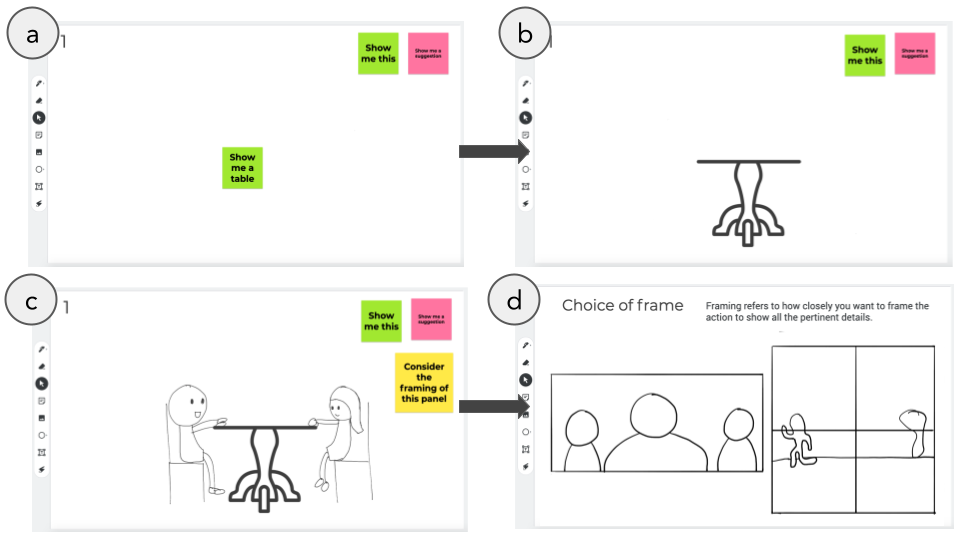
\includegraphics[width=\textwidth]{shown/figures/shown.png}
  \caption[Sh{\"o}wn’s interface and features.]{Sh{\"o}wn’s interface and features. a) A user wants to draw a comic panel showing a table and requests the drawing helper's assistance by typing a sticky note that says, ``Show me a table''. b) The drawing helper then provides a basic icon of the requested object in place of the sticky note request. c) As the user draws their panel, Sh{\"o}wn displays adaptive guidance on the right side of the screen in the form of a sticky note. d) The user can move to the immediate next screen to view relevant examples.}
  \label{fig:shown}
\end{figure}

\subsection{Adaptive Conceptual Guidance: Aiding Showing Relevant \\Examples at Relevant Moments}
We also found in interviews that, while novices enjoyed coming up with their own ideas and stories, they often did not know how to best visualize their ideas. To address this, Sh{\"o}wn provides adaptive conceptual guidance by first presenting high-level comic principles as a suggestion and then specific examples as the user works to inspire ideas for \emph{how} to portray their story. 
The guidance that Sh{\"o}wn currently provides is based on our interviews with experts and three concepts used by experts to decide how to convey a comic story \cite{abel2008drawing,eisner2008comics,mccloud2006making}: choice of framing, choice of moment or transition, and choice of images and words. McCloud \cite{mccloud2006making}, a comic expert and artist, writes that these concepts are part of the ``\textit{rough planning stage where a story’s events are first broken down into readable chunks}'' (\textit{pg. 11}). When presenting guidance, Sh{\"o}wn pairs an explanation of the concept with examples from McCloud’s book that show how the concept can be applied to a comic story.
(The concept of narrative flow is also mentioned in the book, but this refers to panel layout and spacing, which were not applicable to our study as we asked all participants to use the same four-panel layout.) Highlighting the concept behind examples reflects the scenario of an expert guiding a novice through a problem by explaining high-level concepts and providing specific instantiations of the concepts \cite{schon1984reflective}.

The timing of guidance is determined by the following set of recognition heuristics with three principles in mind based on prior work: examples should be related to what the user is currently doing \cite{fraser2019replay,kandel2011wrangler,kumar2011, Lee2010, ngoon2018interactive}, examples should be shown as early in the creative process as possible \cite{kulkarni2012early,Siangliulue}, and examples should be paired with an explanation of the underlying concept they illustrate \cite{javadi2012impact,ngoon2018interactive}.
\\
The three types of guidance that Sh{\"o}wn supports are:

\textbf{Consider the framing for this panel.} Framing refers to composition or use of camera angle and distance to show pertinent actions or details in the panel. This guidance is often presented on the first panel before a user begins drawing to help them get started with their comic. If the user is drawing a subsequent panel, Sh{\"o}wn presents this guidance if the panel’s framing is repeated from any previous panels (\textit{e.g.} if the user begins to use a medium shot in the second panel after using the same camera angle/shot in the first panel). 

\textbf{Consider the moment or transition between panels.} Moment or transition refer to the continuity between actions in panels and the specific moments shown as part of the story in each panel. This guidance is presented when a user moves to a new panel to help them think of transitions between panels.

\textbf{Consider the combination of images and words in this panel.} The combination of images and words refers to how words and images together can tell story more powerfully than either alone. This guidance is presented if the images between panels are similar, if a panel contains a lot of or no text or dialogue, or if the user is attempting to draw facial expressions. 

\subsection{Adaptive Conceptual Guidance in Action}
While the user is drawing their comic, the Wizard is simultaneously using the same prototype link to provide guidance to the user. As the user is drawing their comic, Sh{\"o}wn adaptively displays one of the three guidance suggestions based on the user’s current task and context. The Wizard displays guidance ambiently \cite{matejka2011ambient} on the right side of the panel page without interruption to the user via the sticky notes tool (Figure \ref{fig:shown}c). For instance, a user is drawing the same composition for two panels, in which two people are sitting at a table in the center of the page. Because of the repeated framings, the Wizard presents guidance for the user to ``\textit{consider the framing of this panel}'' in the form of a sticky note that is added to the right side of the drawing screen (Figure \ref{fig:shown}c) to provide inspiration for alternative ways of composing the panel. When the user sees the suggestion and clicks on the sticky note, the Wizard displays a specific example screen that shows examples corresponding to the concept being presented (Figure \ref{fig:shown}d). The user can then return to their drawing screen and modify their drawing if they choose. When the user moves to the next panel, the Wizard presents guidance for the user to ``\textit{consider the moment or transition between panels}'' before the user begins to draw their panel. After clicking on the sticky note, the Wizard presents examples showing different ways to use pacing in a comic narrative. Users can also proactively ask for guidance at any point by clicking the ``Show me a suggestion'' sticky note on the right side of any drawing screen. Users can also ignore guidance if they choose.

\subsection{The Drawing Helper: Freeing Focus from Detail}
In our interview study, novices experienced difficulty in executing their ideas and overly focused on details due to a lack of confidence in their drawing skills. To mitigate this and enable a larger focus on story, Sh{\"o}wn provides a drawing helper that can automatically render a basic sketch of a requested object using Google Jamboard's Autodraw feature, which presents icons that match the sketch input. We differentiate these icons from examples presented in adaptive conceptual guidance as these are basic renderings of objects rather than conceptual examples. If the options provided by Autodraw were not sufficient, the human Wizard provided a simple drawn sketch. The drawing helper was designed to draw basic objects such as a table or person rather than complex characters or scenes. For instance, a user wants to draw a comic story about two people having a dinner date. They want to draw the couple sitting at a table, but don't want to focus on the details of the table itself. The user asks the drawing helper for a table by making a sticky note with the text ``\textit{show me a table},'' and placing it in the center of the drawing screen (Figure \ref{fig:shown}a). The Wizard then produces an icon of the table in the location specified by the user (Figure \ref{fig:shown}b). Later, the user wants a drawing of a chair and this time requests an example via voice command by saying ``show me a chair.'' Sh{\"o}wn renders an icon of a chair, and the user can move the chair to where they desire on the screen. The drawing helper provides simple drawing objects so the user can then focus their attention on utilizing the conceptual examples that support the high-level narrative aspects of their comic story.